%% Kapitel Funktionen
%% GESO-Kompendium
%% philipp.freimann@bbw.ch
%%

\renewcommand{\kAufgabenBuchstabe}{F}

\deu{\section{Funktionen}\index{Funktionen}}
\eng{\section{Functions}\index{Functions}}
\setcounter{aufgabenNummer}{200}

\kMatheNinjaLink{\deu{Funktionen}\eng{Functions}}{https://matheninja.ch/funktionen/}


\subsection{\deu{Grundlagen}\eng{Basics}}

%% %%%%%%%%%%%%%%%%%%%%%%% Aufgabe %%%%%%%%%%%%%%%%%%%%%%%%%%%%%%%%%%%%%%%%%%%%%%%%
\kTrainingAufgabe{
\textbf{\deu{Graphen Zeichenen}\eng{Drawing graphs}}:
\deu{Zeichnen Sie den Graphen der Funktion im Bereich}
\eng{Sketch the graph of the function in the range}
$-4 \le{} x \le{} 4$.

a) $y=\frac12\cdot{}x$ \hspace{30mm}
b) $y=\frac1x$ \hspace{30mm}
c) $y=x^2$

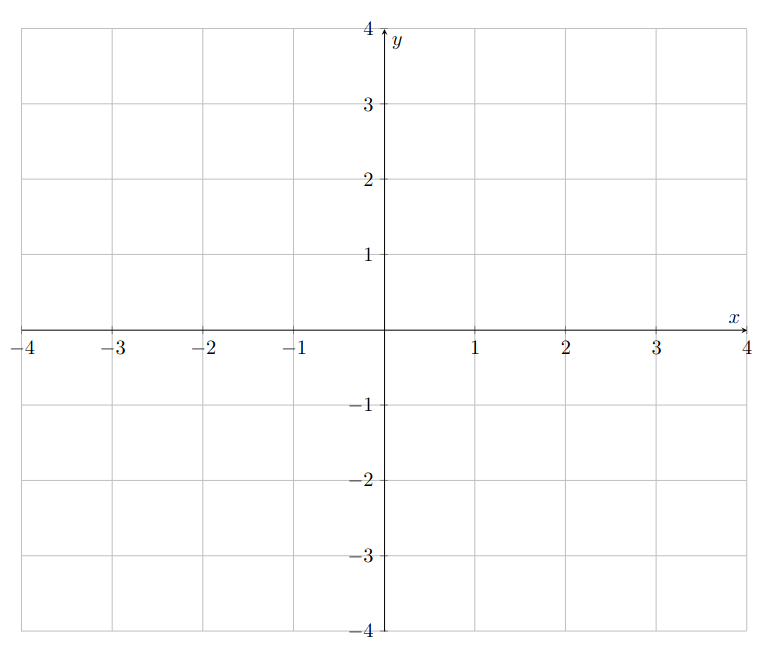
\includegraphics[width=150mm]{img/fct/Fct_ssA01.png}

\kVerweiseAltesKompendium{20}{1}
\kPlatzFuerBerechnungen{6}

}{%% Lösung
\raisebox{-80mm}{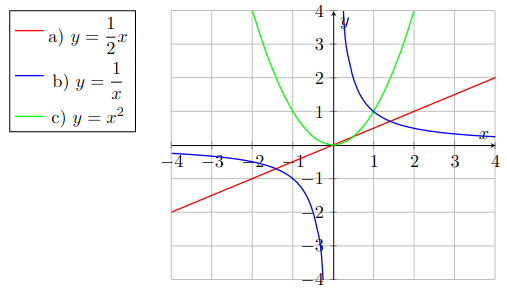
\includegraphics[width=150mm]{img/fct/Fct_ssL01.png}}
}

\kKommentar{Warum haben ab jetzt Aufgaben Titel???}
\kKommentar{Titel vor den Aufgaben}

%% %%%%%%%%%%%%%%%%%%%%%%% Aufgabe %%%%%%%%%%%%%%%%%%%%%%%%%%%%%%%%%%%%%%%%%%%%%%%%

\kTrainingAufgabe{

  Füllen Sie die folgende Wertetabelle zu gegebenen Funktion aus:

  $$f(x) =  \frac{-3}2\cdot{} x + \frac14$$

  \begin{tabular}{c|c|c|c|c|c|c}\hline
 $x$    & -1 & 0 & 1 & 2 & 3 & 4\\\hline
 $f(x)$ &   &  &  &   &   & 
  \end{tabular}
  
  \kKommentar{Neue Aufgabe (Niveau)}
}{%% Lösungen
}
%% %%%%%%%%%%%%%%%%%%%%%%% Aufgabe %%%%%%%%%%%%%%%%%%%%%%%%%%%%%%%%%%%%%%%%%%%%%%%%


\kTrainingAufgabe{
\textbf{\deu{Funktionen auswerten}\eng{Evaluate the function}}:
\deu{Werten Sie den Funktionsterm $y=x^2-2x-5$ für folgende $x$-Werte aus:}
\eng{Evaluate the function term $y=x^2-2x-5$ for the following $x$-values:}

a) $\frac12$ \hspace{25mm}
b) $-1$ \hspace{25mm}
c) $-\frac12$ \hspace{25mm}
d) $-\frac34$ \hspace{25mm}
\kVerweiseAltesKompendium{20}{2}
\kPlatzFuerBerechnungen{6}

}{%% Lösung
a) $-\frac{23}4$ \hspace{25mm}
b) $-2$ \hspace{25mm}
c) $-\frac{15}{4}$ \hspace{25mm}
d) $-\frac{47}{16}$ \hspace{25mm}
}



\subsection{\deu{Lineare Funktionen}\eng{Linear Functions}}

%% %%%%%%%%%%%%%%%%%%%%%%% Aufgabe %%%%%%%%%%%%%%%%%%%%%%%%%%%%%%%%%%%%%%%%%%%%%%%%
\kTrainingAufgabe{
\textbf{\deu{Steigungsbegriff, Mittelpunkt einer Strecke}\eng{Slope concept, midpoint of a line segment}}:

\kKommentar{Mittelpunkt ist ein geometrisches Konzept.}
\kKommentar{Kommt im Rahmenlehrpln \textbf{nicht} vor?}

a) \deu{Bestimmen Sie die Steigungen der Strecken a bis i. Zeichnen Sie
Steigungsdreiecke ein.}
\eng{Determine the slopes of the line segments a to i. Draw slope triangles.}

b) \deu{Bestimmen Sie die Koordinaten des Mittelpunkts jeder Strecke.}
\eng{Determine the coordinates of the midpoint of each line segment.}

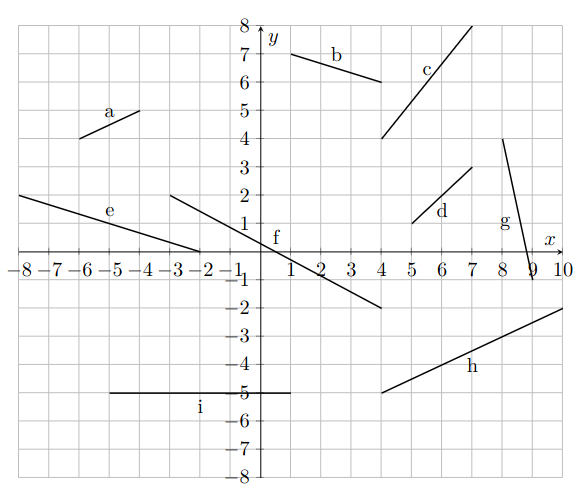
\includegraphics[width=130mm]{img/fct/Fct_ssA03.png}
\kVerweiseAltesKompendium{20}{3}
\kPlatzFuerBerechnungen{6}

}{%% Lösung

\renewcommand{\arraystretch}{2}
\begin{tabular}{|c|c|c|c|c|c|c|c|c|c|}\hline
   & a & b &c &d &e &f &g &h &i\\\hline
$a=m=$ & $\frac12$ & $\frac{-1}3$ & $\frac43$ & $1$ & $\frac{-1}3$
& $\frac{-4}7$ & $-5$ & $\frac12$ & $0$\\\hline
M.: & $(-5|\frac92)$ & $(\frac52|6.5)$ & $(5.5|6)$ & $(6|2)$ &
$(-5|1)$ & $(\frac12|0)$ & $(8.5|\frac32)$ & $(7|\frac{-7}2)$ & $(-2|-5)$\\\hline
 \end{tabular}
\renewcommand{\arraystretch}{2}
 
}%% end Aufgabe


%% %%%%%%%%%%%%%%%%%%%%%%% Aufgabe %%%%%%%%%%%%%%%%%%%%%%%%%%%%%%%%%%%%%%%%%%%%%%%%
\kTrainingAufgabe{
\textbf{\deu{Graph zeichnen, Achsenschnittpunkte einzeichnen}\eng{Draw the graph, mark intercepts}}:
\deu{Zeichnen Sie die Graphen folgender Funktionen und heben Sie den Schnittpunkt mit der $y$-Achse und die
Nullstelle hervor.}%% end deu

\eng{Draw the graphs of the following functions and emphasize the $y$-axis intercept and the zero point.}

a) $y=2x+1$ \hspace{25mm}
b) $y=-x+3$ \hspace{25mm}
c) $y=-0.5x+4$ \hspace{25mm}

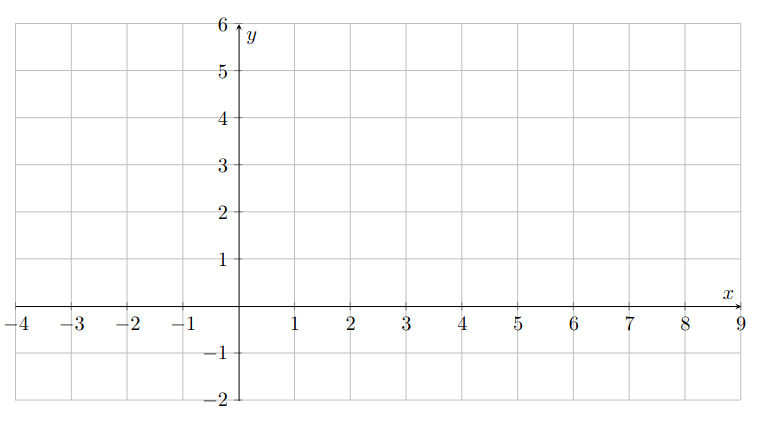
\includegraphics[width=150mm]{img/fct/Fct_ssA04.png}
\kVerweiseAltesKompendium{21}{4}
\kPlatzFuerBerechnungen{6}


}{%% Lösung

\raisebox{-50mm}{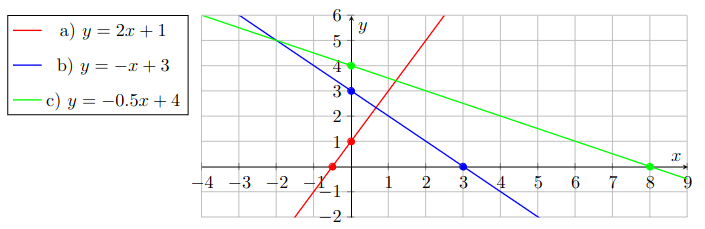
\includegraphics[width=150mm]{img/fct/Fct_ssL04.png}}

}



%% %%%%%%%%%%%%%%%%%%%%%%% Aufgabe %%%%%%%%%%%%%%%%%%%%%%%%%%%%%%%%%%%%%%%%%%%%%%%%
\kTrainingAufgabe{
\textbf{\deu{Funktionsterm auswerten:}\eng{Evaluate function expression}}
\deu{Werten Sie die Funktion $f(x) = 2x+1$ für folgende Argumente  aus:}
\eng{Evaluate the function $f(x) = 2x+1$ for the following arguments:}

$2$, $-2$, $0.5$, $-0.5$.
\kVerweiseAltesKompendium{21}{5}
\kPlatzFuerBerechnungen{6}

}{%% Lösung
$f(2)= 5$ \hspace{10mm}
$f(-2)=-3$ \hspace{10mm}
$f(0.5) = 2$ \hspace{10mm}
$f(-0.5)=0$
}




%% %%%%%%%%%%%%%%%%%%%%%%% Aufgabe %%%%%%%%%%%%%%%%%%%%%%%%%%%%%%%%%%%%%%%%%%%%%%%%
\kTrainingAufgabe{
\textbf{\deu{Bedeutung der Parameter; explizite Form:}\eng{Meaning of parameters; explicit form:}}

\deu{Bestimmen Sie Steigung und $y$-Achsenabschnitt in der durch die Funktionsgleichung $3x-2y=60$ gegebenen Geraden.}
\eng{Determine the slope and $y$-intercept in the line given by the equation $3x-2y=60$.}
\kVerweiseAltesKompendium{21}{6}
\kPlatzFuerBerechnungen{6}

}{%% Lösung
  
$$y = 1.5x - 30$$
\deu{Steigung}\eng{Slope} = +1.5 \eng{and}\deu{und} $y$-\deu{Achsenabschnitt}\eng{intercept} = -30.
}





%% %%%%%%%%%%%%%%%%%%%%%%% Aufgabe %%%%%%%%%%%%%%%%%%%%%%%%%%%%%%%%%%%%%%%%%%%%%%%%
\kNiveauAufgabe{
\textbf{\deu{Achsenschnittpunkte berechnen:}\eng{Calculate intercepts:}}
  
  \deu{Berechnen Sie die Achsenschnittpunkte der Geraden $g$ mit der Funktionsgleichung $y=-0.25x+4$.}
  \eng{Calculate the intercepts of the line $g$ with the functional equation $y=-0.25x+4$.}
\kVerweiseAltesKompendium{21}{7}
\kPlatzFuerBerechnungen{6}


}{%% Lösung
\deu{Mit $x$-Achse:}\eng{With $x$-Axis:} $(0|4)$

\deu{Mit $y$-Achse:}\eng{With $y$-Axis:} $(16|0)$
}


%% %%%%%%%%%%%%%%%%%%%%%%% Aufgabe %%%%%%%%%%%%%%%%%%%%%%%%%%%%%%%%%%%%%%%%%%%%%%%%
\kTrainingAufgabe{
\textbf{\deu{Horizontale Gerade}\eng{Horizontal line}}:
\deu{Notieren Sie die Funktionsgleichung der horizontalen Geraden
  durch den Punkt}%...
\eng{Write down the functional equation of the horizontal line passing
  through the point}%...
 $P=(5|8)$.
\kVerweiseAltesKompendium{21}{8}
\kPlatzFuerBerechnungen{6}

}{%% Lösung
$f(x) = y = 8$
}




%% %%%%%%%%%%%%%%%%%%%%%%% Aufgabe %%%%%%%%%%%%%%%%%%%%%%%%%%%%%%%%%%%%%%%%%%%%%%%%
\kTrainingAufgabe{
\textbf{\deu{Zweipunkteaufgabe}\eng{Two-point problems}:}

\deu{Wie lautet die Funktionsgleichung der Geraden, die durch folgende
  zwei Punkte läuft (Resultate exakt angeben)?}
\eng{What is the functional equation of the line passing through the following two points (provide exact results)?}

a) $A(5|8)$ \deu{und}\eng{and} $B(7|12)$


b) $A(-3|4)$ \deu{und}\eng{and} $B(2|1)$


c) $A(-1|1)$ \deu{und}\eng{and} $B(10|5)$

\kKommentar{ev zu simpel, da mit TR lin-reg möglich}
\kVerweiseAltesKompendium{21}{9}
\kPlatzFuerBerechnungen{6}


}{%% Lösung
TR: lin-reg

a) $A=(5|8)$ \deu{und}\eng{and} $B=(7|12)$ $\Longrightarrow$  $y=2x-2$


b) $A=(-3|4)$ \deu{und}\eng{and} $B=(2|1)$ $\Longrightarrow$ $y=\frac{-3}5x+\frac{11}5$


c) $A=(-1|1)$ \deu{und}\eng{and} $B=(10|5)$ $\Longrightarrow$  $y=\frac4{11}x+\frac{15}{11}$
}




%% %%%%%%%%%%%%%%%%%%%%%%% Aufgabe %%%%%%%%%%%%%%%%%%%%%%%%%%%%%%%%%%%%%%%%%%%%%%%%
\kTrainingAufgabe{
  \textbf{\deu{Funktionsgleichung aus Grafik bestimmen}\eng{Determine the functional equations from the graph}}:
  
  \deu{Wie lauten die Funktionsgleichungen der Geraden $a$ bis $f$?}
  \eng{What are the functional equations of the lines $a$ to $f$?}

\kKommentar{Niveau Aufnahmeprüfung!}

\kKommentar{Gitterpunkte markieren}

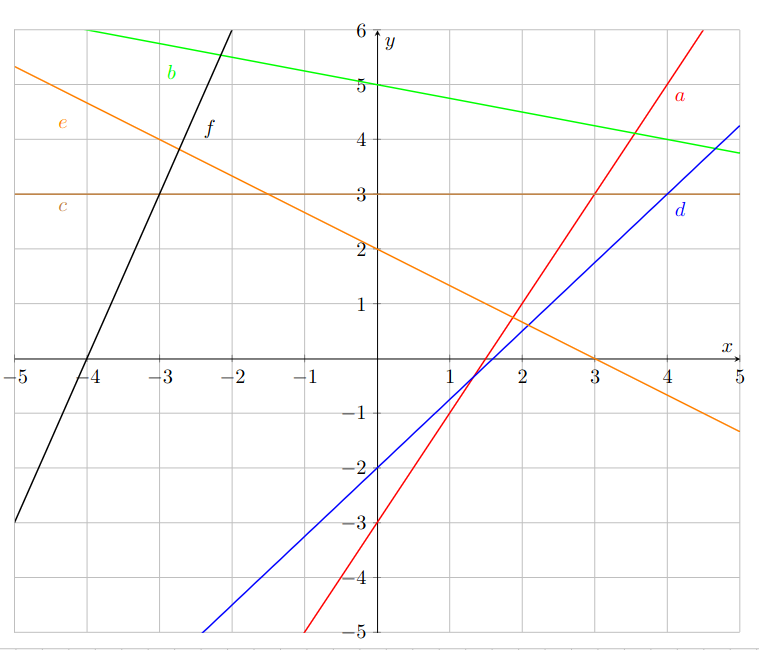
\includegraphics[width=140mm]{img/fct/Fct_ssA10.png}
\kVerweiseAltesKompendium{22}{10}
\kPlatzFuerBerechnungen{6}


}{%% Lösung
\raisebox{-80mm}{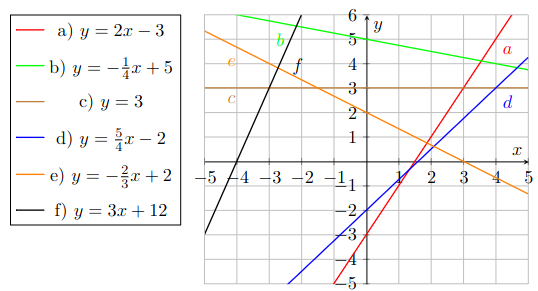
\includegraphics[width=160mm]{img/fct/Fct_ssL10.png}}
}





%% %%%%%%%%%%%%%%%%%%%%%%% Aufgabe %%%%%%%%%%%%%%%%%%%%%%%%%%%%%%%%%%%%%%%%%%%%%%%%
\kNiveauAufgabe{
\textbf{\deu{Achsenschnittpunkte berechnen}\eng{Calculate intercepts}}:
\deu{Berechnen Sie die Schnittpunkte des Graphen mit den beiden
  Koordinatenachsen.}

\eng{Calculate the intercepts of the graph with both coordinate axes.}

\kKommentar{Erste Aufgabe in Grundform gebracht.}

a) $y=3x+10$ \hspace{30mm}
b) $y=5-\frac12x$ \hspace{30mm}
c) $y=\frac{10x-2}5$ 
\kVerweiseAltesKompendium{22}{11}
\kPlatzFuerBerechnungen{6}

}{%% Lösung

\renewcommand{\arraystretch}{2}
\begin{tabular}{c|c|c|c}
& a) $y=10-3x$ & b) $y=5-\frac12x$ & c) $y=\frac{10x-2}5$  \\\hline
$N(x_n|0)$ & $\left(\frac{10}3\middle|0\right)$ & $(10|0)$ &
$(\frac15|0)$ \\\hline
$B(0|b)$ & $(0|10)$ & $(0|5)$ & $\left(0\middle|\frac{-5}2\right)$
 \end{tabular}
 
\renewcommand{\arraystretch}{2}

}





%% %%%%%%%%%%%%%%%%%%%%%%% Aufgabe %%%%%%%%%%%%%%%%%%%%%%%%%%%%%%%%%%%%%%%%%%%%%%%%

\kTrainingAufgabe{
\textbf{\deu{Umwandeln in die explizite Form}\eng{Convert to explicit form}}:

\deu{Wandeln Sie die Funktionsgleichung in die explizite Form $y=ax+b$ (bzw. $y=mx+q$) um.}
\eng{Convert the function equation into explicit form $y=ax+b$ (or $y=mx+q$).}

\kKommentar{Besser Bestimmen Sie Steigung und $y$-Achseabschnitt}

\kKommentar{Titel ändern oder weglassen.}

a) $y=2-\frac{x}2$

b) $y=\frac{2x-10}3$

c) $y=\frac{1-x}{12}$

d) $y = -(2+1.25x)$

e) $4y-3x = 1.5$
\kVerweiseAltesKompendium{22}{12}
\kPlatzFuerBerechnungen{6}

}{%% Lösung

a) $y=\frac{-1}2\cdot{}x + 2$

b) $y=\frac23\cdot{}x - \frac{10}3$

c) $y=\frac{-1}{12}\cdot{}x + \frac1{12}$

d) $y=\frac{-5}4\cdot{}x - 2$

e) $y=\frac34\cdot{}x + \frac38$
}




%% %%%%%%%%%%%%%%%%%%%%%%% Aufgabe %%%%%%%%%%%%%%%%%%%%%%%%%%%%%%%%%%%%%%%%%%%%%%%%

\kNiveauAufgabe{
\textbf{\deu{Liegt $P (-4.5|7)$ auf, oberhalb oder unterhalb der Geraden $g$?}\eng{Is $P(-4.5, 7)$ located on, above, or below the line $g$?}}

\kKommentar{Jede der drei Varianten soll vorkommen.}

a) $g: y=-2x-2$

b) $g: y= -0.5x + 4.7$

c) $g: y = 2.5x + 18.25$
\kVerweiseAltesKompendium{23}{13}
\kPlatzFuerBerechnungen{6}

}{%% Lösung

\deu{a) Punkt liegt \textbf{auf} der Geraden.  

b) Punkt liegt \textbf{oberhalb} der Geraden.  

c) Punkt liegt \textbf{auf} der Geraden.  }%% end deutsch

\eng{
a) Point lies \textbf{on} the line.

b) Point lies \textbf{above} the line.

c) Point lies \textbf{on} the line.}%% end english
}


%% %%%%%%%%%%%%%%%%%%%%%%% Aufgabe %%%%%%%%%%%%%%%%%%%%%%%%%%%%%%%%%%%%%%%%%%%%%%%%


\kNiveauAufgabe{
\deu{\textbf{Geradengleichung aus Steigung und einem Punkt $P \in g$ (Punkt-Steigungs-Aufgabe)}}

\eng{\textbf{Equation of a line from slope and a point $P \in g$ (Point-slope problem)}}

\deu{Eine Gerade $g$ hat die Steigung $-0.4$ und geht durch $P (-2| -7)$. Wie lautet
  die Funktionsgleichung von $g$?}

\eng{A line $g$ has a slope of $-0.4$ and passes through $P (-2| -7)$. What is the
  equation of the line $g$?}%% end eng
\kVerweiseAltesKompendium{23}{14}
\kPlatzFuerBerechnungen{6}

\kKommentar{Erst eine Aufgabe positiv: a=4 P(10|42)}


}{%% Lösung
$g : y = -0.4x - 7.8$
}



%% %%%%%%%%%%%%%%%%%%%%%%% Aufgabe %%%%%%%%%%%%%%%%%%%%%%%%%%%%%%%%%%%%%%%%%%%%%%%%

\kNiveauAufgabe{
\deu{\textbf{Liegen drei gegebene Punkte auf einer gemeinsamen Geraden oder nicht?}}
\eng{\textbf{Do three given points lie on a common line or not?}}

\kKommentar{nötig??}

\deu{Liegen $A(-2.5| -20.8)$, $B(21.5|50.0)$ und $C(100.0|281.575)$ auf
  einer gemeinsamen Geraden $g$ oder nicht? Begründung?}
\eng{Do $A(-2.5| -20.8)$, $B(21.5|50.0)$, and $C(100.0|281.575)$ lie on
a common line $g$ or not? Justification?}
\kVerweiseAltesKompendium{23}{15}
\kPlatzFuerBerechnungen{6}


}{%% Lösung
\deu{Ja, die Steigung von $AB$ ist gleich der Steigung von $BC$,
  nämlich $2.95$.}
\eng{es, the slope of $AB$ is equal to the slope of $BC$,
which is $2.95$.}
}

\kKommentar{Neue Aufgabe:}

\kTrainingAufgabe{Wie lautet eine lineare Funktionsgleichung, welche
  die Gerade beschreibt, die durch die Punkte $A(4|9.5)$ und $B(-1|-3)$ verläuft.}{%% Lösung:
 $$y=2.5x-0.5$$
}
\kTrainingAufgabe{Wie lautet eine lineare Funktionsgleichung, welche
  die Gerade beschreibt, die durch die Punkte $A(3|-1)$ und $B(-3|-19)$ verläuft.}{%% Lösung:
 $$y=3x-10$$
}

\kTrainingAufgabe{Wie lautet eine lineare Funktionsgleichung, welche
  die Gerade beschreibt, die durch die Punkte $A(2|0.5)$ und $B(-3|1.75)$ verläuft.}{%% Lösung:
 $$y= -0.25x+1$$
}

%% %%%%%%%%%%%%%%%%%%%%%%% Aufgabe %%%%%%%%%%%%%%%%%%%%%%%%%%%%%%%%%%%%%%%%%%%%%%%%

\kNiveauAufgabe{
  \deu{\textbf{Fehlende Punktkoordinate bestimmen:}}
  \eng{\textbf{Determine the missing coordinate:}}

  \deu{
Der Punkt $C(-12.5|y_C)$ liegt auf der Geraden
$g$ durch $A(-2.5| - 20.8)$ und $B(21.5|50.0)$. Wie lautet die
Koordinate $y_C$?}%% end deutsch
  \eng{The point $C(-12.5|y_C)$ lies on the line
$g$ through $A(-2.5| - 20.8)$ and $B(21.5|50.0)$. What is the coordinate $y_C$?}

 \kVerweiseAltesKompendium{23}{16}
\kPlatzFuerBerechnungen{6}

 
}{%% Lösung

$y_C = -50.3$
}


%% %%%%%%%%%%%%%%%%%%%%%%% Aufgabe %%%%%%%%%%%%%%%%%%%%%%%%%%%%%%%%%%%%%%%%%%%%%%%%


\kNiveauAufgabe{
\deu{\textbf{Geradengleichung einer zur gegebenen Geraden parallelen Geraden durch einen
    Punkt bestimmen:}}
\eng{\textbf{Determine the equation of a line parallel to the given line and passing through a point:}}

\eng{Given $g: y = 4.8x - 2$. The line $h$ is parallel to $g$ and passes through the point $P(-8|2)$. What is the equation of $h$?}
\deu{Gegeben ist $g : y = 4.8x - 2$. Die Gerade $h$ ist parallel zu $g$ und läuft
durch den Punkt $P(-8|2)$. Wie lautet die Geradengleichung von $h$?}
\kVerweiseAltesKompendium{23}{17}
\kPlatzFuerBerechnungen{6}

}{%% Lösung
$h : y = 4.8x + 40.4$
}


%% %%%%%%%%%%%%%%%%%%%%%%% Aufgabe %%%%%%%%%%%%%%%%%%%%%%%%%%%%%%%%%%%%%%%%%%%%%%%%

\kNiveauAufgabe{
\deu{\textbf{Schnittpunkt S zweier Geraden berechnen}}:
\eng{\textbf{Calculate the intersection point SS of two lines}}:


\deu{Berechnen Sie den Schnittpunkt von $g: \frac{-2}3x+5$ und $h:  \frac{-3}4x+10$.}
\eng{Calculate the intersection point of $g: \frac{-2}3x+5$ and $h:  \frac{-3}4x+10$.}
\kVerweiseAltesKompendium{23}{18}
\kPlatzFuerBerechnungen{6}

}{%% Lösung
\deu{Schnittpunkt}\eng{Intersection} = $(180|125)$
}



\deu{\textbf{Kombinationen obiger Grundaufgaben}}
\eng{\textbf{Combinations of the basic problems above}}

\kNiveauAufgabe{
\deu{Die Gerade $g$ hat die Steigung $-0.5$ und die Nullstelle bei $x = 5$. Wie lautet die Funktionsgleichung von $g$?}
\eng{The line $g$ has a slope of $-0.5$ and the $x$-intercept at $x = 5$. What is the equation of $g$?}
\kVerweiseAltesKompendium{24}{19}
\kPlatzFuerBerechnungen{6}

}{%% Lösung
$g : y = -0.5x + 2.5$
}


%% %%%%%%%%%%%%%%%%%%%%%%% Aufgabe %%%%%%%%%%%%%%%%%%%%%%%%%%%%%%%%%%%%%%%%%%%%%%%%


\kNiveauAufgabe{
\deu{Die Gerade $g$ hat die Steigung $-3$. Ferner liegt $A(-2|4)$ auf $g$. Der Punkt $B(x_B | - 23)$ liegt
  ebenfalls auf $g$. Wie lautet die Koordinate $x_B$?}
\eng{The line $g$ has a slope of $-3$. Additionally, the point $A(-2|4)$ lies on $g$. The point $B(x_B | -23)$ also lies on $g$. What is the coordinate $x_B$?}
\kVerweiseAltesKompendium{24}{20}
\kPlatzFuerBerechnungen{6}


}{%% Lösung
$x_B = 7$
}


%% %%%%%%%%%%%%%%%%%%%%%%% Aufgabe %%%%%%%%%%%%%%%%%%%%%%%%%%%%%%%%%%%%%%%%%%%%%%%%

\kNiveauAufgabe{
\deu{Die Gerade $g$ geht durch $A(1|5)$ und $B(8| - 2)$. Die Gerade $h$ schneidet die $x$-Achse im
selben Punkt $N$ wie die Gerade $g$. Die Gerade $h$ hat ferner die Steigung $4$. Wie lautet die
Funktionsgleichung von $h$?}
\eng{The line $g$ passes through $A(1|5)$ and $B(8| - 2)$. The line $h$ intersects the $x$-axis at the same point $N$ as line $g$. Furthermore, the line $h$ has a slope of $4$. What is the functional equation of $h$?}
\kVerweiseAltesKompendium{24}{21}
\kPlatzFuerBerechnungen{6}

}{%% Lösung
$h : y = 4x - 24$
}


\deu{\textbf{Angewandte lineare Funktionen}}
\eng{\textbf{Applied linear functions}}

%% %%%%%%%%%%%%%%%%%%%%%%% Aufgabe
%% %%%%%%%%%%%%%%%%%%%%%%%%%%%%%%%%%%%%%%%%%%%%%%%%
\kNiveauAufgabe{

  Beim einem Taxianbieter kostet eine Fahrt von 6 km total 32 Fr. (Grundgebühr + Kilometertarif) und eine Fahrt von 9 km kostet insgesamt 45.50 Fr. 

a) Bestimme die Funktionsgleichung, mit der sich die Kosten in Abhängigkeit der Fahrstrecke berechnen lassen. 

b) Wie viel kostet eine Fahrt von 11 km? 
  
  \kKommentar{neue Aufgabe}
}{%% Lösung
a)  $$y= 4.5  \cdot{} x   + 5$$

b)  $$54.50 CHF$$
}

\kNiveauAufgabe{
  
\deu{Eine Taxifahrt von 10 km kostet CHF 21, eine solche von 15 km aber CHF 27. Wie lautet
die lineare Funktionsgleichung $y = f (x)$ mit $x$ = Anzahl km Fahrstrecke und $y$ = Anzahl CHF
Gesamttaxe? Variante: Gesucht die Funktionsgleichung $K = f (s)$, $K$ = Kosten in CHF, $s$ =
Strecke in km. Es werden beide Varianten akzeptiert.}
\eng{The linear functional equation for the taxi fare is given by $y = f(x)$, where $x$ is the distance traveled in kilometers and $y$ is the total fare in CHF. Alternatively, the functional equation can be expressed as $K = f(s)$, where $K$ is the cost in CHF and $s$ is the distance in kilometers. Both variants are acceptable.}
\kVerweiseAltesKompendium{24}{22}
\kPlatzFuerBerechnungen{6}


}{%% Lösung

$y = 1.2x + 9 $

  \deu{oder (Variante)}
  \eng{or (variant)}

$K(s) = 1.2 \text{CHF/km} · s + 9 \text{CHF}$

}%% end Aufgabe



%% %%%%%%%%%%%%%%%%%%%%%%% Aufgabe %%%%%%%%%%%%%%%%%%%%%%%%%%%%%%%%%%%%%%%%%%%%%%%%
\kKommentar{Schwierige Aufgabe Celcius/Fahrenheit verschoben}

%% %%%%%%%%%%%%%%%%%%%%%%% Aufgabe %%%%%%%%%%%%%%%%%%%%%%%%%%%%%%%%%%%%%%%%%%%%%%%%


\kNiveauAufgabe{
\deu{Eine lineare Notenskala ist wie folgt festgelegt:
  Für 24 Punkte gibt es Note 6, für 0 Punkte Note 1.}

\eng{A linear grading scale is defined as follows:
For 24 points, the grade is 6, and for 0 points, the grade is 1.}

\deu{
a) Wie lautet die lineare Notenfunktion $y = f (x)$? $x$ = Anzahl Punkte, $y$ = Notenzahl.

b) Welche Note (auf eine Dezimalen gerundet) wird mit 18 Punkten erreicht?

c) Wie viele Punkte ergeben die Note 4?}%% end deu


\eng{}%% end eng
a) What is the linear grading function $y=f(x)$;  $x$= Number of points, $y$ = Grade.

b) Which grade (rounded to one decimal place) is achieved with 18 points?

c) How many points result in a grade of 4?
\kVerweiseAltesKompendium{24}{24}
\kPlatzFuerBerechnungen{6}

}{%% Lösung

a) $y=\frac5{24}x+1$

b) $4.8$

c) 14.4 Punkte
}




%% %%%%%%%%%%%%%%%%%%%%%%% Aufgabe %%%%%%%%%%%%%%%%%%%%%%%%%%%%%%%%%%%%%%%%%%%%%%%%
\kNiveauAufgabe{

\deu{Lineare \textbf{Abschreibung} einer Maschine: Eine Maschine mit
  Neuwert CHF 5\,000.- wird linear abgeschrieben: Jedes Jahr soll sich
  ihr Wert um CHF 250.- verringern.}%% end edu

\eng{Linear \textbf{Depreciation} of a Machine: A machine with an
  initial value of CHF 5\,000.- is depreciated linearly: Its value is
  supposed to decrease by CHF 250 every year.}%% end eng
  

\deu{
  a) Wie lautet die lineare Abschreibungsfunktion $y = f (x)$ mit $x$ = Anzahl Jahre und $y$ =
Anzahl CHF Zeitwert nach $x$ Jahren?

b) Nach wie vielen Jahren ist die Maschine vollständig
abgeschrieben?}%% end deu

\eng{
  a) What is the linear depreciation function $y=f(x)$ with $x$ being the number of years and $y$ being the value in CHF after $x$ years?

b) After how many years is the machine fully depreciated?
}%% end eng

\kVerweiseAltesKompendium{25}{25}
\kPlatzFuerBerechnungen{6}

}{ %% Lösung
a) $y = -250x + 5000$

b) \deu{Nach 20 Jahren.} \eng{After 20 years.}
}%% end kNiveauAufgabe



%% %%%%%%%%%%%%%%%%%%%%%%% Aufgabe %%%%%%%%%%%%%%%%%%%%%%%%%%%%%%%%%%%%%%%%%%%%%%%%

\kNiveauAufgabe{
\deu{Für HD-TV via Internet wird neben einer Grundgebühr auch die Anzahl Stunden, während
derer man fernsieht, verrechnet. Anbieter A verlangt pro Monat eine Grundgebühr von CHF
5.- und pro Stunde fernsehen eine Gebühr von 20 Rappen. Anbieter B verlangt folgendes:
Bei 20 h fernsehen CHF 10.- und bei 100 h fernsehen CHF 20.- (beides inkl. Grundgebühr).
Wie lauten die beiden Kostenfunktionen? $x$ = Anzahl Stunden Fernsehzeit, $y$ = Anzahl CHF
Kosten. Bei welcher Stundenzahl sind beide Anbieter gleich teuer?}

\eng{For HD-TV via the internet, in addition to a basic fee, the number of hours spent watching is also charged. Provider A charges a monthly basic fee of CHF 5 and a fee of 20 cents per hour of watching. Provider B charges as follows: CHF 10 for 20 hours of watching and CHF 20 for 100 hours of watching (both including the basic fee). What are the two cost functions? $x$ = Number of hours of TV time, $y$ = Number of CHF costs. At what number of hours are both providers equally expensive?}

\kVerweiseAltesKompendium{25}{26}
\kPlatzFuerBerechnungen{6}

}{%% Lösung
  \deu{Gleicher Preis bei 33 Stunden und 20 Minuten.}
  \eng{They are equally expensive after 33 hours and 20 minutes.}
}

%% %%%%%%%%%%%%%%%%%%%%%%% Aufgabe %%%%%%%%%%%%%%%%%%%%%%%%%%%%%%%%%%%%%%%%%%%%%%%%


\kNiveauAufgabe{
  \newcommand{\tempGrad}[1]{${}^{\circ{}}$#1}
  \deu{Die englische Temperaturskala (Fahrenheit-Grade, \tempGrad{F}) ist wie folgt festgelegt:
0\tempGrad{C} (Celsius) entsprechen 32 \tempGrad{F} (Fahrenheit). 100 \tempGrad{C}
entsprechen 212 \tempGrad{F}.}

  \eng{The English temperature scale (Fahrenheit degrees, \tempGrad{F}) is defined as follows: 0\tempGrad{C} (Celsius) corresponds to 32 \tempGrad{F} (Fahrenheit), and 100 \tempGrad{C} corresponds to 212 \tempGrad{F}.}

a) \deu{Wie lautet die lineare Funktionsgleichung zur Umrechnung von \tempGrad{C} (= $x$) in \tempGrad{F} (= $y$)?}
   \eng{What is the linear function equation for converting \tempGrad{C} (= $x$) to \tempGrad{F} (= $y$)?}
b) \deu{Wie lautet die lineare umgekehrte Funktion zur Umrechnung von \tempGrad{F}(= $x$) in \tempGrad{C} (= $y$)?}
   \eng{What is the linear inverse function for converting \tempGrad{F}(= $x$) to \tempGrad{C} (= $y$)?}
\kVerweiseAltesKompendium{24}{23}
\kPlatzFuerBerechnungen{6}

}{%% Lösung
a) $y = 1.8x + 32$

b) $y= \frac95 x - \frac{160}9$
}




\subsubsection{Grafisches Lösen von Gleichungssystemen}

\kKommentar{Hier einfachere Aufgaben. Die sind alle 4 blöd.}

\kKommentar{Besser 1-2 Aufgaben, die aufgehen.}

\kKommentar{Beispiel: y=2x-5 und y=-x+4 schnitt (3|1)}

\kKommentar{Beispiel: 2y=x+12 und y=2x+3 schnitt (2|7)}

\deu{Lösen Sie jeweils das Gleichungssystem grafisch und interpretieren Sie die
  Lösung:}
\eng{Solve each system of equations graphically and interpret the solution:}

%% %%%%%%%%%%%%%%%%%%%%%%% Aufgabe %%%%%%%%%%%%%%%%%%%%%%%%%%%%%%%%%%%%%%%%%%%%%%%%


\kNiveauAufgabe{\gleichungZZ{3x-4y}{8}{y}{\frac14 x + 6}

\begin{center}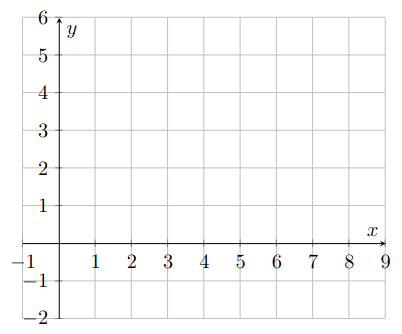
\includegraphics[width =
    100mm]{img/fct/Fct_ssA27a.png}\end{center}
\kVerweiseAltesKompendium{25}{27}
\kPlatzFuerBerechnungen{6}
}{\gleichungZZ{3x-4y}{8}{y}{\frac14 x + 6} $$S=(8|4)$$

\begin{center}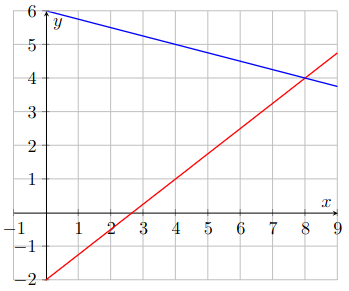
\includegraphics[width = 100mm]{img/fct/Fct_ssL27a.png}\end{center}
}

%% %%%%%%%%%%%%%%%%%%%%%%% Aufgabe %%%%%%%%%%%%%%%%%%%%%%%%%%%%%%%%%%%%%%%%%%%%%%%%



\kNiveauAufgabe{  
   \gleichungZZ{10y}{7.5x}{18.75x+25y}{1500}\begin{center}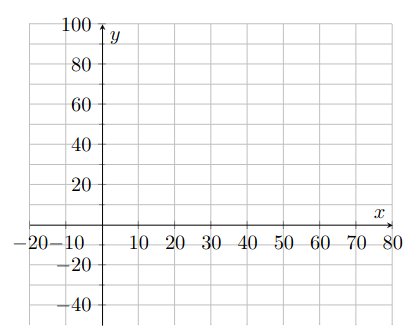
\includegraphics[width = 100mm]{img/fct/Fct_ssA27b.png}\end{center}
\kVerweiseAltesKompendium{15}{39}
\kPlatzFuerBerechnungen{6}
}{\gleichungZZ{10y}{7.5x}{18.75x+25y}{1500} $$S=(40|30)$$

  \begin{center}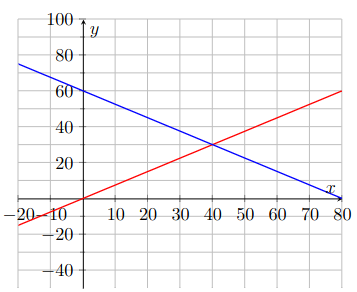
\includegraphics[width=100mm]{img/fct/Fct_ssL27b.png}\end{center}
}

%% %%%%%%%%%%%%%%%%%%%%%%% Aufgabe %%%%%%%%%%%%%%%%%%%%%%%%%%%%%%%%%%%%%%%%%%%%%%%%


\kNiveauAufgabe{  
 \gleichungZZ{3x+y-9.5}{4y-\frac{28}7}{-\frac45y+x}{-5+0.2x}

\begin{center}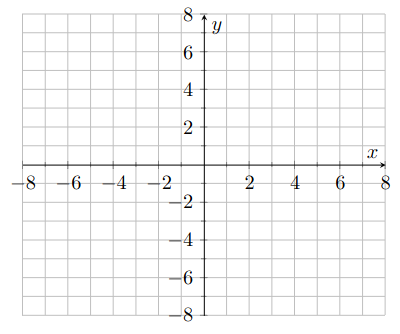
\includegraphics[width=100mm]{img/fct/Fct_ssA27c.png}\end{center}
\kVerweiseAltesKompendium{15}{40}
\kPlatzFuerBerechnungen{6}
}{\gleichungZZ{13x+y-9.5}{4y-\frac{28}7}{-\frac45y+x}{-5+0.2x}

$$\mathbb{L}_S = \left\{\right\}$$

\begin{center}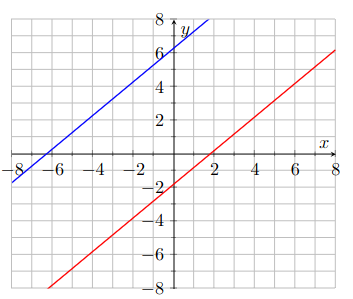
\includegraphics[width = 100mm]{img/fct/Fct_ssL27c.png}\end{center}

}


%% %%%%%%%%%%%%%%%%%%%%%%% Aufgabe %%%%%%%%%%%%%%%%%%%%%%%%%%%%%%%%%%%%%%%%%%%%%%%%

\kNiveauAufgabe{  
 \gleichungZZ{40}{-2y-x}{3.5x-5y+82}{4\left(x-y+\frac{51}2\right)}

\begin{center}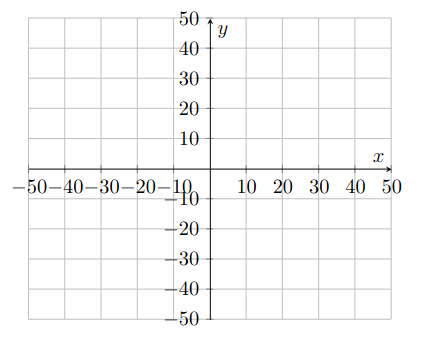
\includegraphics[width = 100mm]{img/fct/Fct_ssA27d.png}\end{center}
\kVerweiseAltesKompendium{15}{41}
\kPlatzFuerBerechnungen{6}
}{ \gleichungZZ{40}{-2y-x}{3.5x-5y+82}{4\left(x-y+\frac{51}2\right)}

\deu{Die Geraden sind zusammenfallend.}\eng{The lines coincide.}

$$\mathbb{L}_{(x|y)} = \{(x|y) \in \mathbb{R}\times\mathbb{R} | y=\frac{-x}2 - 20\}$$

\begin{center}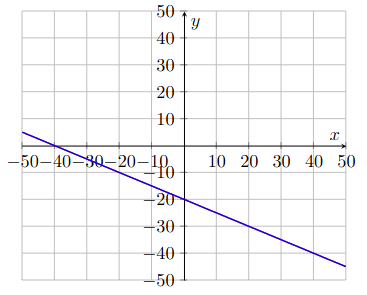
\includegraphics[width = 100mm]{img/fct/Fct_ssL27d.png}\end{center}

}%% end Aufgabe

\newpage






\subsection{\deu{Potenzfunktionen}\eng{Power Functions}}

\kMatheNinjaLink{\deu{Potenzfunktionen}\eng{Power Functions}}{https://matheninja.ch/potenzfunktionen/}

\kKommentar{Titel nun korrekt: (nicht  Hyperbelfunktion etc.)}

\subsubsection{$n>1$: \deu{Parabeln}\eng{Parabolas}}



%% %%%%%%%%%%%%%%%%%%%%%%% Aufgabe %%%%%%%%%%%%%%%%%%%%%%%%%%%%%%%%%%%%%%%%%%%%%%%%

\kNiveauAufgabe{
\deu{Zeichnen Sie den Graphen folgender Potenzfunktionen:}
\eng{Draw the graph of the following power functions:}
a) $x \mapsto 0.5x^3$  \hspace{30mm}  b) $x\mapsto -x^4$

\begin{tabular}{cc}
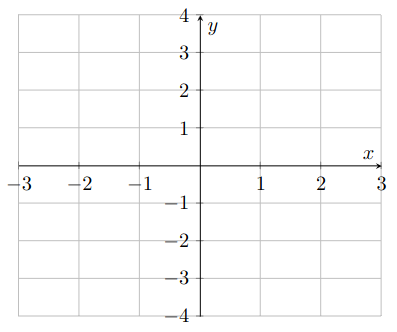
\includegraphics[width=85mm]{img/fct/Fct_ssA28a.png}
&
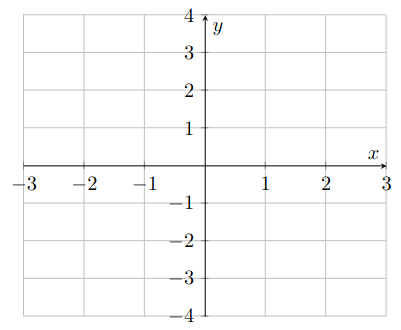
\includegraphics[width=85mm]{img/fct/Fct_ssA28b.png}
\\
 \end{tabular}
 
\kVerweiseAltesKompendium{26}{28}
\kPlatzFuerBerechnungen{6}

}{%% Lösung

\begin{tabular}{cc}
a)

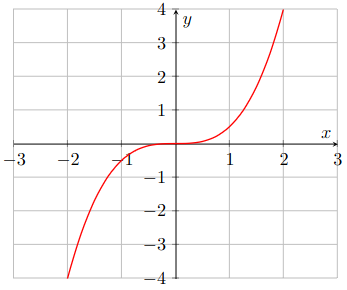
\includegraphics[width=70mm]{img/fct/Fct_ssL28a.png}
&b)

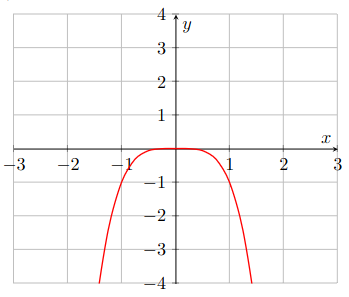
\includegraphics[width=70mm]{img/fct/Fct_ssL28b.png}
\\
 \end{tabular}
}



%% %%%%%%%%%%%%%%%%%%%%%%% Aufgabe %%%%%%%%%%%%%%%%%%%%%%%%%%%%%%%%%%%%%%%%%%%%%%%%

\kNiveauAufgabe{
\deu{Bestimmen Sie den Faktor $a$ in $x\mapsto a\cdot{}x^4$ wenn der Graph durch den Punkt $A(2|3)$ verläuft.}
\eng{Determine the factor $a$ in $x\mapsto a \cdot x^4$ when the graph
passes through the point $A(2|3)$.}
\kVerweiseAltesKompendium{26}{29}
\kPlatzFuerBerechnungen{6}
}{%% Lösung
$3=a\cdot{}2^4 \Longrightarrow a=\frac3{16}$
}%% end KNiveauAufgabe


\kNiveauAufgabe{
\deu{Bestimmen Sie den Faktor $a$ in $x\mapsto a\cdot{}x^5$ wenn der Graph durch den Punkt $A(-3|48.6)$ verläuft.}
\eng{Determine the factor $a$ in $x\mapsto a \cdot x^5$ when the graph
passes through the point $A(-3|48.6)$.}
\kKommentar{neue Aufgabe}
\kPlatzFuerBerechnungen{6}
}{%% Lösung
$48.6=a\cdot{}(-3)^5 \Longrightarrow a=-\frac15$
}%% end KNiveauAufgabe


\kNiveauAufgabe{
\deu{Bestimmen Sie den Exponenten der Funktion $y=x^n$, wenn der Graph
  durch den Punkt
  $A=(3|6561)$ verläuft.}
\eng{translate}
\kKommentar{neue Aufgabe}
\kPlatzFuerBerechnungen{6}
}{%% Lösung
  $6561 = 3^n \Longrightarrow n=\log_3(6561) = 8$
}%% end KNiveauAufgabe




\kKommentar{ev. Punkteaufgabe, duch logarithmieren.}



\subsubsection{$n < 0$
  \deu{Hyperbeln}\eng{Hyperbolas}}\deu{\index{Hyperbeln}} \eng{\index{Hyperbolas}}


%% %%%%%%%%%%%%%%%%%%%%%%% Aufgabe %%%%%%%%%%%%%%%%%%%%%%%%%%%%%%%%%%%%%%%%%%%%%%%%

\kNiveauAufgabe{
\deu{Bestimmen Sie den Faktor $a$ der Potenzfunktion $y=a\cdot{}x^{-3}$,
wenn der Graph dieser Hyperbel durch den Punkt
$A\left( 3 \middle| \frac1{54} \right)$ verläuft.}
\eng{Determine the factor $a$ of the power function $y = a \cdot x^{-3}$ when the graph of this hyperbola passes through the point $A\left(3 \middle| \frac{1}{54}\right)$.}
\kVerweiseAltesKompendium{26}{30}
\kPlatzFuerBerechnungen{6}

}{%% Lösungs
$\frac1{54}=a\cdot{}3^{-3} \Longrightarrow   a=27\cdot{}\frac1{54} = \frac12$
}



%% %%%%%%%%%%%%%%%%%%%%%%% Aufgabe %%%%%%%%%%%%%%%%%%%%%%%%%%%%%%%%%%%%%%%%%%%%%%%%

\kNiveauAufgabe{
\deu{Welche Funktion gehört zu welchem Graphen? Ordnen Sie die Zahl dem Buchstaben zu.}
\eng{Which function belongs to which graph? Match the number to the letter.}

a) $y = -x^3$  \hspace{15mm}  b) $y=x^{-2}$  \hspace{15mm} c)
$y=3\cdot{}x^{-1}$ \hspace{15mm}  d) $y=-0.5x^4$

\begin{center}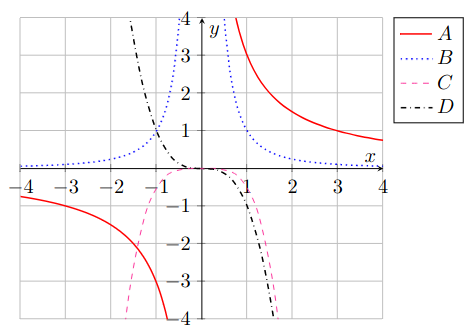
\includegraphics[width=150mm]{img/fct/Fct_ssA31.png}\end{center}
\kVerweiseAltesKompendium{26}{31}
\kPlatzFuerBerechnungen{6}


}{%% Lösung
a) $y = -x^3$  \hspace{15mm}  b) $y=x^{-2}$  \hspace{15mm} c)
$y=3\cdot{}x^{-1}$ \hspace{15mm}  d) $y=-0.5x^4$

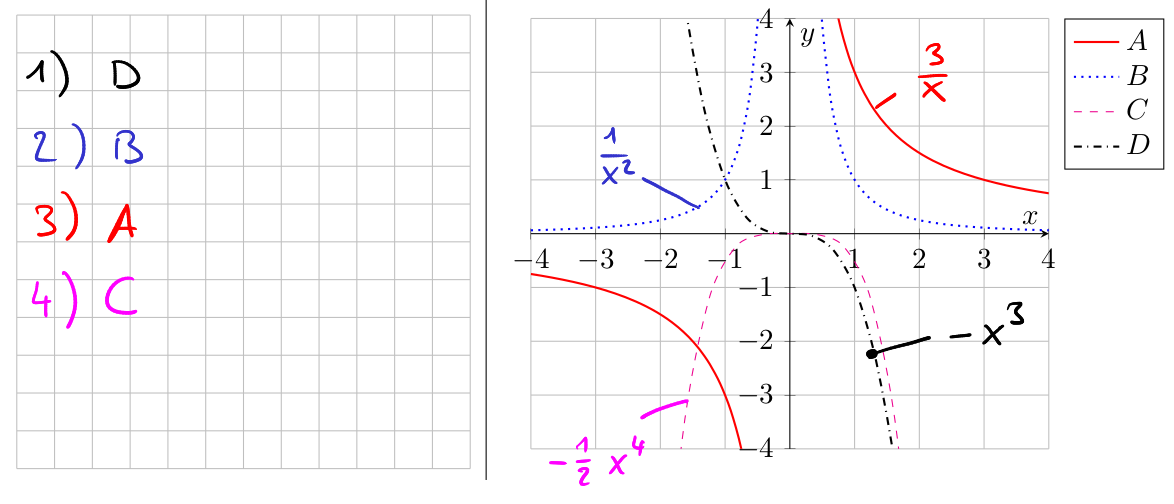
\includegraphics[width=150mm]{img/fct/Fct_ssL31.png}

}

\newpage






\newcommand{\e}{\text{e}}%% eulersche Zahl e \ne Variable e

\subsection{\deu{Exponentialfunktionen}\eng{Exponential functions}}

\subsubsection{\deu{Exponentielle Prozesse, Exponentialfunktion}\eng{Exponential processes, exponential function}}

\textbf{\deu{Wachstums und Zerfallsprozesse}}
\textbf{\eng{Growth and decay processes}}

%% %%%%%%%%%%%%%%%%%%%%%%% Aufgabe %%%%%%%%%%%%%%%%%%%%%%%%%%%%%%%%%%%%%%%%%%%%%%%%

\kNiveauAufgabe{
\deu{Zinseszins; Entwicklung eines Startkapitals bei konstantem Jahreszinssatz: Ein
Kapital von CHF 100.- wird über viele Jahre zu einem konstanten
\eng{Zinssatz von 2\% verzinst.}Compound interest; development of an initial capital with a constant annual interest rate: A capital of CHF 100.- is compounded over many years at a constant interest rate of 2\%.}

\begin{enumerate}[label=\alph*)]
\item
\deu{Bestimmen Sie den Zinsfaktor.}\eng{Bestimmen Sie den Zinsfaktor.}
\item
\deu{Wie lautet die Funktion $K = f (t)$, $K$ = Kapital zur Zeit $t$,
$t$ = Zeit in Jahren?}
\eng{What is the function $K = f(t)$, where $K$ is the capital at time $t$, and $t$ is the time in years?}

\item
\deu{Stellen Sie die Kapitalentwicklung grafisch dar}%
\eng{Graphically represent the capital development}:
$0 \le t \le 320$.
\end{enumerate}

\begin{center}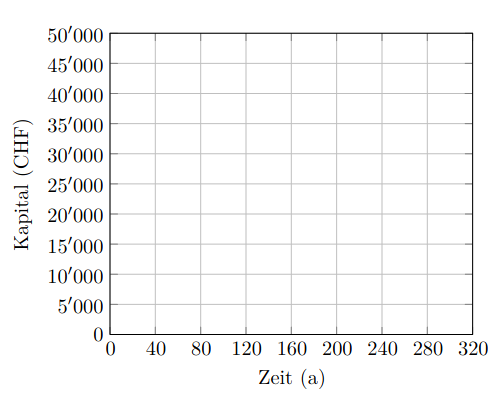
\includegraphics[width=150mm]{img/fct/Fct_ssA32.png}\end{center}
\kVerweiseAltesKompendium{27}{32}
\kPlatzFuerBerechnungen{6}


}{%% Lösung
\begin{enumerate}[label=\alph*)]
\item
Der Zinsfaktor ist $1.02$.
\item
$K = f (t) = 100\cdot 1.02^t$, $t$ = Zeit in Jahren?
\item
\deu{S. folgende Grafik}
\eng{consult the following graphic}
\end{enumerate}
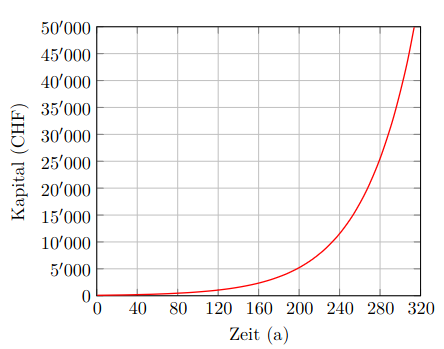
\includegraphics[width=150mm]{img/fct/Fct_ssL32.png}

}%% end Aufgabe



%% %%%%%%%%%%%%%%%%%%%%%%% Aufgabe %%%%%%%%%%%%%%%%%%%%%%%%%%%%%%%%%%%%%%%%%%%%%%%%


\kNiveauAufgabe{
\deu{Degressive Abschreibung:}\eng{Declining depreciation:}

\deu{Eine Maschine mit einem Neuwert von CHF 20\,000.- wird degressiv abgeschrieben. Sie verliert jährlich 10\% an Wert.}
\eng{A machine with an initial value of CHF 20\,000 is depreciated in a declining manner. It loses 10\% of its value annually.}

\begin{enumerate}[label=\alph*)]
\item
\deu{Bestimmen Sie den Abnahmefaktor.}
\eng{Determine the depreciation factor.}
\item
\deu{Erstellen Sie eine Wertetabelle: $t$ = Zeit in Jahren, $W=f(t)$ = Wert Maschine zur Zeit $t$.}
\eng{Create a value table: $t$ = time in years, $W=f(t)$ = value of the machine at time $t$.}
\item
\deu{Stellen Sie die Werte-Entwicklung grafisch dar: $0 \le t \le 10$.}
\eng{Graphically represent the value development: $0 \le t \le 10$.}
\item
\deu{Wie lautet eine möglicher Funktionsterm zu $W=f(t)$?}
\eng{What is a possible function term for $W=f(t)$?}
\end{enumerate}

\begin{center}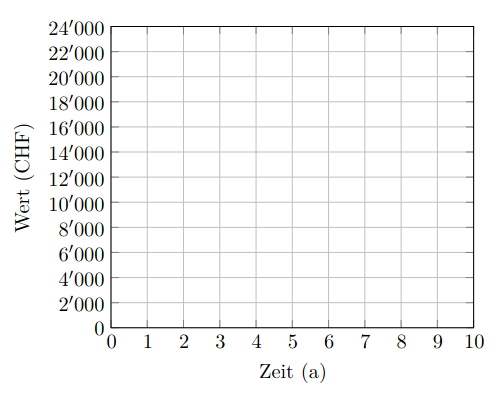
\includegraphics[width=150mm]{img/fct/Fct_ssA33.png}\end{center}
\kVerweiseAltesKompendium{27}{33}
\kPlatzFuerBerechnungen{6}


}{%% Lösungen
\begin{enumerate}[label=\alph*)]
\item
\deu{Der Abnahmefaktor (hier Abschreibungsfaktor) ist}\eng{The
depreciation factor is}
$100\%-10\% = (100-10)\% = 90\% = 90\cdot{}\frac1{100} = 0.9$
\item
\begin{tabular}{|c|c|c|c|c|c|}\hline
\deu{Jahr}\eng{Year}    & 0 & 1 & 2 & 3 & 4 \\\hline
\deu{Wert}\eng{Value}   & 20\,000 & 18\,000 & 16\,200 & 14\,580 & 13\,122 \\\hline
 \end{tabular}
 
\item
\deu{S. folgende Graphik}
\eng{consult the following graphic}
\end{enumerate}

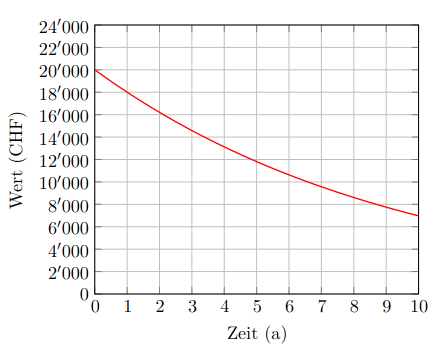
\includegraphics[width=150mm]{img/fct/Fct_ssL33.png}

}

%% %%%%%%%%%%%%%%%%%%%%%%% Aufgabe %%%%%%%%%%%%%%%%%%%%%%%%%%%%%%%%%%%%%%%%%%%%%%%%

\kTrainingAufgabe{
\deu{Prozentuale Wachstumsrate $\leftrightarrow$ Wachstumsfaktor}%
\eng{Percentage growth rate $\leftrightarrow$ Growth factor}:

\deu{Suchen Sie zu folgenden prozentualen Wachstumsraten den
zugehörigen Wachstumsfaktor}%
\eng{Find the corresponding growth factor for the following percentage growth rates}:

a) Rate = $4\%$
\hspace{15mm}
b) Rate = $2.2\%$
\hspace{15mm}
c) Rate = $0.5\%$
\kVerweiseAltesKompendium{27}{34}
\kPlatzFuerBerechnungen{6}

}{%% Lösungen

a) $1.04$ 
\hspace{15mm}
b) $1.022$
\hspace{15mm}
c) $1.005$
}

%% %%%%%%%%%%%%%%%%%%%%%%% Aufgabe %%%%%%%%%%%%%%%%%%%%%%%%%%%%%%%%%%%%%%%%%%%%%%%%

\kTrainingAufgabe{
\deu{Prozentuale Abnahmerate $\leftrightarrow$ Abnahmefaktor: Suchen Sie zu folgenden prozentualen
Abnahmeraten den zugehörigen Abnahmefaktor:}

\eng{Percentage decrease rate $\leftrightarrow$ Decrease factor:
Find the corresponding decrease factor for the following percentage
decrease rates:}

a) Rate = $4\%$
\hspace{15mm}
b) Rate = $20\%$
\hspace{15mm}
c) Rate = $5.5\%$
\kVerweiseAltesKompendium{28}{35}
\kPlatzFuerBerechnungen{6}

}{%% Lösungen

a) $0.96$ 
\hspace{15mm}
b) $0.8$
\hspace{15mm}
c) $0.945$
}



%% %%%%%%%%%%%%%%%%%%%%%%% Aufgabe %%%%%%%%%%%%%%%%%%%%%%%%%%%%%%%%%%%%%%%%%%%%%%%%
\kNiveauAufgabe{
\deu{\textbf{Graphen von Exponentialfunktionen:}}
\eng{\textbf{Graphs of Exponential Functions:}}

\deu{Zeichnen Sie die Graphen von $f(x) = 2^x$ und $g(x) = 2^{-x}$ im
Bereich $-3 \le x \le 3$.}

\eng{Draw the graphs of $f(x) = 2^x$ and $g(x) = 2^{-x}$ in the range $-3 \le x \le 3$.}

\deu{
a) Vergleichen Sie die beiden Graphen. Wo schneiden sich die Graphen?

b) Bestimmen Sie Definitionsbereich und Wertebereich der beiden Funktionen.

c) Haben die Funktionen Nullstellen? Haben Sie Asymptoten?
}

\eng{
a) Compare the two graphs. Where do the graphs intersect?

b) Determine the domain and range of both functions.

c) Do the functions have roots? Do they have asymptotes?
}

\bbwGraph{-4}{4}{-1}{9}{}

\kVerweiseAltesKompendium{28}{36}
\kPlatzFuerBerechnungen{6}

}{%% Lösung


\begin{center}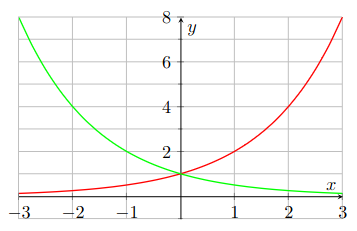
\includegraphics[width=150mm]{img/fct/Fct_ssL36.png}\end{center}

\deu{a) Die Graphen sind spiegelsymmetrisch (gespiegelt an der
$y$-Achse. Sie schneiden sich im Punkt $(0|1)$.

b) Definitonsbereich $\definitionsmenge = \mathbb{R}$ und Wertebereich
$\mathbb{W} = \mathbb{R}^{+}\backslash \{0\}$.

c) Die Funktionen haben keine Nullstellen, da der Wertebereich
$\mathbb{R}^+\backslash{}\{0\}$ ist. Der Funktions\textbf{wert} Null
kommt also nicht vor.

Für beide Funktionen ist die $x$-Achse die Asymptote.
}%% end deutsch

\eng{
a) The graphs are symmetric (reflected across the $y$-axis). They intersect at the point $(0|1)$.

b) Domain $\definitionsmenge = \mathbb{R}$ and range $\mathbb{W} = \mathbb{R}^{+}\backslash {0}$.

c) The functions have no roots since the range is $\mathbb{R}^+\backslash{}{0}$. The function value zero is not present.

For both functions, the $x$-axis is the asymptote.
}%% end english
}




%% %%%%%%%%%%%%%%%%%%%%%%% Aufgabe %%%%%%%%%%%%%%%%%%%%%%%%%%%%%%%%%%%%%%%%%%%%%%%%


\kNiveauAufgabe{
\deu{Nennen Sie eine mögliche Exponentialfunktion $f(x) = a^x$ [bzw. $a^\frac{x}{\tau}$] (also mit $f(0)=1$), bei der sich der Funktionswert

a) verdoppelt, wenn man das Argument um 3 erhöht (siehe Abbildung),

\begin{center}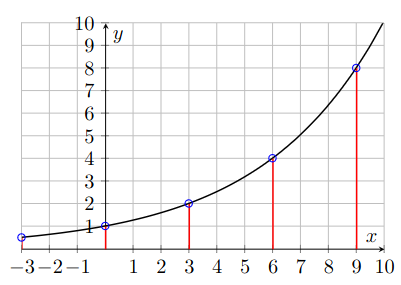
\includegraphics[width=65mm]{img/fct/Fct_ssA37.png}\end{center}

b) verdoppelt, wenn man $x$ um 12 erhöht bzw.

c) halbiert, wenn man $x$ um 12 erhöht.}%% end deutsch

\eng{Give a possible exponential function $f(x) = a^x$ [or $a^\frac{x}{\tau}$] (with $f(0)=1$) where the function value

a) doubles when the argument is increased by 3 (see figure),

\begin{center}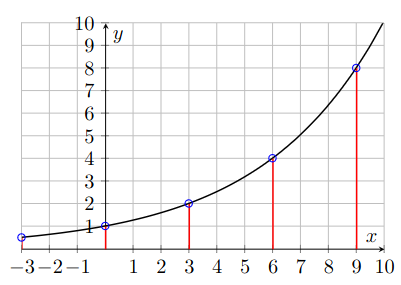
\includegraphics[width=85mm]{img/fct/Fct_ssA37.png}\end{center}

b) doubles when $x$ is increased by 12, or

c) halves when $x$ is increased by 12.}%% end engl

\kVerweiseAltesKompendium{28}{37}
\kPlatzFuerBerechnungen{6}

}{%% Lösung


a) $f(x) = 2^\frac{x}3 =  \left(2^\frac13\right)^x =\left(\sqrt[3]{2}\right)^x$

b) $f(x) = 2^\frac{x}{12} =  \left(2^\frac1{12}\right)^x
=\left(\sqrt[12]{2}\right)^x $

b) $f(x) = \left(\frac12\right)^\frac{x}{12} =  \left(\left(\frac12\right)^\frac1{12}\right)^x
=\left(\sqrt[12]{\frac12}\right)^x $

}

%% %%%%%%%%%%%%%%%%%%%%%%% Aufgabe %%%%%%%%%%%%%%%%%%%%%%%%%%%%%%%%%%%%%%%%%%%%%%%%

\kNiveauAufgabe{
\deu{
a) Die Wachstumsrate der Bevölkerung in der Schweiz betrug im Jahr 2012 ca. 1.1\%. 2012
zählte die Schweiz 8\,039\,100 Einwohner. Wie viele Personen werden bei gleich bleibender
Wachstumsrate im Jahr 2030 in der Schweiz leben (auf 100 Personen
genau)?

b) Seit 1999 wächst die Wohnbevölkerung der Stadt Zürich wieder. Im Jahr 1999 zählte die
Stadt Zürich 360\,704 Einwohner, im Jahr 2012 waren es 394\,012 Personen. Berechnen Sie
die durchschnittliche jährliche Wachstumsrate in \% (Genauigkeit: 2 Dezimalen). (Zum
Vergleich: Im Jahr 2012 betrug die Wachsumsrate 1\%.)}%% end deutsch

\eng{
a) The population growth rate in Switzerland was approximately 1.1\%
in 2012.
In 2012, Switzerland had a population of 8\,039\,100. How many people will live in Switzerland in 2030 with a constant growth rate (rounded to 100 people)?

b) Since 1999, the resident population of the city of Zurich has been
growing again. In 1999, the city of Zurich had 360,704 inhabitants,
and in 2012, there were 394\,012 people.
Calculate the average annual growth rate in percent (accuracy: 2
decimals). (For comparison: In 2012, the growth rate was 1\%.)}%% end english
\kVerweiseAltesKompendium{29}{38}
\kPlatzFuerBerechnungen{6}


}{%% Lösungen

a) $8\,039\,100 \cdot{} 1.011^t$ \deu{mit}\eng{with} $t=2030-2012=18$ is\deu{t} $9\,788\,800$.

b) $\Delta\tau = 2012-1999 = 13$

\deu{Wachstumsfaktor}\eng{Growth factor}:
$$q^{13} = \frac{394\,012}{360\,704} \Longrightarrow
q=\sqrt[13]{...}\approx 1.0068$$

\deu{Somit beträgt die jährliche Wachstumsrate ca. }
\eng{So, the annual growth rate is about }
0.68\%.
}%% end aufgabe

\kKommentar{Luftdruck: Aufgabe 39. aus altem Komp. gestrichen???}
\kKommentar{Warum?}

%% %%%%%%%%%%%%%%%%%%%%%%% Aufgabe %%%%%%%%%%%%%%%%%%%%%%%%%%%%%%%%%%%%%%%%%%%%%%%%
\kNiveauAufgabe{
  
\deu{Berechnen Sie die durchschnittliche jährliche Wachstumsrate in \% für die Bevölkerung einer
Stadt, die innert 10 Jahren von 70\,000 Personen auf 82\,000 Personen angewachsen ist. (Genauigkeit: 1 Dezimale.)}%% end deu

\eng{Calculate the average annual growth rate in percent for the
population of a city that has grown from 70\,000 to 82\,000 within 10
years. (Accuracy: 1 decimal place.)}%% end eng

\kVerweiseAltesKompendium{29}{40}
\kPlatzFuerBerechnungen{6}

}{%% Lösung
$\Delta\tau = 10$; 
\deu{somit gilt für den Wachstumsfaktor
$q^{10} = \frac{82\,000}{70\,000}$. Der Faktor ist daher $q=\sqrt[10]{\frac{82}{70}} \approx 1.0159$. Die
prozentuale Zunahme (Rate) gerundet in Prozent ist also: 1.6\%.}%% end
%% deutsch

\eng{therefore, the growth factor is given by:

  $q^{10} = \frac{82\,000}{70\,000}$
  
Hence, the factor $q$ is approximately
$q=\sqrt[10]{\frac{82}{70}} \approx 1.0159$. The rounded percentage
increase (rate) is approximately 1.6\%.}%% end eng

}%% end Aufgabe



%% %%%%%%%%%%%%%%%%%%%%%%% Aufgabe %%%%%%%%%%%%%%%%%%%%%%%%%%%%%%%%%%%%%%%%%%%%%%%%

\kNiveauAufgabe{

\kKommentar{Aufgabe geändert, da Begriff Eindringtiefe schon vergeben}

\kKommentar{Eindringtiefe $d= 1/\ln(a)$ mit $a$=Abnahmefaktor pro cm.}

\deu{Licht, das durch eine Glasplatte der Dicke $d$ geht, verliert an Intensität $I$. 
Pro eingedrungenen cm verliert das Licht bei einer bestimmten
Glassorte 60\% seiner Intensität. Die
Anfangsintensität beträgt 100 Watt/m${}^2$.}%% end deu

\eng{Light passing through a glass plate of thickness dd loses
  intensity II. For each penetrated centimeter, the light loses 60\% of its intensity for a particular type of glass. The initial intensity is 100 Watts/m${}^2$.}

\deu{a) Bestimmen Sie eine mögliche Funktionsgleichung $I = f(d)$, für $I$ =
Intensität in W/m${}^2$ und $d$ = cm der Eindringung.

b) Bestimmen Sie die Intensität nach 5 cm im Glas. (Genauigkeit 3 Dezimalen.)

c) Nach wie vielen cm im Glas beträgt die Lichtintensität noch 1/100
der Anfangsintensität? (Genauigkeit: auf mm genau.)}%% end deu


\eng{
a) Determine a possible function equation I=f(d)I=f(d), where II is the intensity in W/m22 and dd is the depth of penetration in cm.

b) Determine the intensity after 5 cm in the glass. (Precision: 3 decimal places.)

c) At how many centimeters into the glass is the light intensity only
1/100 of the initial intensity? (Precision: exact to the nearest
millimeter.)}%% end eng


\kVerweiseAltesKompendium{30}{41}
\kPlatzFuerBerechnungen{6}


}{%% Lösungen

a) $I = f(d) =
100\cdot{}0.4^d \left[\frac{\text{Watt}}{\text{m}^2}\right]$

b)  $f(5) = 0.4^5 = 1.024 \left[\frac{\text{Watt}}{\text{m}^2}\right]$

c) $\log_{0.4}\left(\frac1{100}\right) \approx 5.026$ cm. \deu{Gerundet}\eng{Rounded}: 50 mm
}

%% %%%%%%%%%%%%%%%%%%%%%%% Aufgabe %%%%%%%%%%%%%%%%%%%%%%%%%%%%%%%%%%%%%%%%%%%%%%%%

\kNiveauAufgabe{

%%In einer Probe werden 13.5 mg radioaktives Material gemessen. Pro Tag nimmt die Menge des radioaktiven Stoffes um 11 % ab. Wie lautet die Zerfallsfunktion? Wie viel des radioaktiven Stoffs sind nach 8 Tagen noch vorhanden? Wann sind weniger als 0.1 mg des Stoffs vorhanden? 

In einem Wald verbreitet sich ein schädliches Unkraut
exponentiell. Pro Tag nimmt die bewachsene Fläche um 0.5 \% zu. Zu Beginn sind 5.6 m${}^2$ bewachsen. Wie lautet die Wachstumsfunktion? Wie viel Fläche ist nach 120 Tagen bewachsen? Wann sind mehr als 100 m${}^2$ bewachsen? 
  \kKommentar{neue Aufgaeb}
}{%% lösung
  a) $y = 5.6 \cdot{} 1.005^t$ ($t$ in Tagen)

  b) $y = ... ?? Nachrechnen!!$

  \kKommentar{Nachrechnen}
}


%% %%%%%%%%%%%%%%%%%%%%%% Aufgabe
%% %%%%%%%%%%%%%%%%%%%%%%%%%%%%%%%%%%%%%%%%%%%%%%%


\kNiveauAufgabe{}{% Lösunrg
  \eng{translate}


  Ein Computervirus in einem Netzwerk verbreitet sich gemäss der folgenden Funktion: 

$f(x) = 18762\cdot{}e^{0.331\cdot{}t}$, mit $t$ = Zeit in Tagen, gemessen ab heute und $f(t)$ = Anzahl infizierter Computer 

 
a) Berechne die Anzahl infizierter Computer nach 14 Tagen. 

b) Berechne die prozentuale Zunahme pro Woche. 

c) Wann hat sich die Anzahl infizierter Computer im Vergleich zu heute
verzehnfacht?

  \kKommentar{neue Aufgabe}
}{%% lösungen

}

%% %%%%%%%%%%%%%%%%%%%%%%% Aufgabe %%%%%%%%%%%%%%%%%%%%%%%%%%%%%%%%%%%%%%%%%%%%%%%%

\kNiveauAufgabe{
\deu{Bei der Radio-Iodtherapie kommt radioaktives ${}^{131}$Iod zum Einsatz. Von anfänglich 20.000 mg
  Substanz sind nach 7 Tagen noch 10.289 mg vorhanden.}%% end deu
\eng{In radioiodine therapy, radioactive ${}^{131}$iodine is used. Initially, there were 20,000 mg of the substance, and after 7 days, only 10,289 mg are still present.}


\deu{
a) Wie lautet eine Zerfallsfunktion $m = f(t)$, für  $m$ = Masse in g,
und $t$ = Zeit in Tagen?


b) Bestimmen Sie die Halbwertszeit von ${}^{131}$Iod auf 2 Dezimalen
genau.}%% end deu

\eng{
a) The decay function is given by m=f(t)m=f(t), where mm is the mass in grams, and tt is the time in days.

b) Determine the half-life of ${}^{131}$Iod to two decimal places.}%% end eng

\kVerweiseAltesKompendium{30}{42}
\kPlatzFuerBerechnungen{6}
}{%Lösung (en)

a) \deu{Exakte Formen:}\eng{exact forms:}

$$f(t) = 20.000\cdot{}\left(\frac{10.289}{20.000}\right)^\frac{t}7$$
$$f(t) = 20.000 \cdot{}
e^\frac{\ln\left(\frac{10.289}{20.000}\right)\cdot{}t}{7}$$

\deu{Annäherungen:}\eng{aproximations}

$$f(t) \approx{}  20\cdot{} 0.51445^\frac{t}7 $$
$$f(t) \approx{}  20\cdot{} 0.9094^t $$
$$f(t) \approx{}  20\cdot{} \e^{\frac{-0.6647\cdot{}t}{7}}$$
$$f(t) \approx{}  20\cdot{} \e^{-0.09495\cdot{}t}$$

b) $t\approx 7.30 $ \deu{Tage}\eng{days}
}

%% %%%%%%%%%%%%%%%%%%%%%%% Aufgabe %%%%%%%%%%%%%%%%%%%%%%%%%%%%%%%%%%%%%%%%%%%%%%%%

\kNiveauAufgabe{
\deu{Um wie viele \% nimmt der Wert einer Maschine bei exponentiellem
Zerfall jährlich ab, wenn ihr Wert nach 4 Jahren
auf die Hälfte gesunken ist? (Genauigkeit: 2 Dezimalen.)}

\eng{By what percentage does the value of a machine decrease annually
  in exponential decay
  if its value has halved after 4 years? (Precision: 2 decimal places.)}
\kVerweiseAltesKompendium{30}{43}
\kPlatzFuerBerechnungen{6}
}{%% Lösung
  \deu{Jährliche Abnahme}
  \eng{Annual decrease} $\approx 15.91\%$
}{8}


\kNiveauAufgabe{
\deu{Bei welchem Zinssatz $p$ in \% verdoppelt sich ein Kapital in 20
Jahren? (Genauigkeit: 2 Dezimalen.)}%% end deu
\eng{At what interest rate $p$ in \% does a capital double in 20
  years? (Precision: 2 decimal places.)}%% end eng
\kVerweiseAltesKompendium{30}{44}
\kPlatzFuerBerechnungen{6}
}{%% Lösung
\deu{Zinssatz}\eng{interest rate}: $\approx 3.53\%$
}


%% %%%%%%%%%%%%%%%%%%%%%%% Aufgabe %%%%%%%%%%%%%%%%%%%%%%%%%%%%%%%%%%%%%%%%%%%%%%%%

\kNiveauAufgabe{
  \deu{
    Bei einer Algenplage wird die befallene Fläche in 3 Monaten verdoppelt. Bei der Entdeckung
beträgt die befallene Fläche 120 m${}^2$ . Wie lautet eine mögliche
Wachstumsfunktion $A = f(t)$ mit 
$A$ = befallene Fläche in m${}^2$, $t$ = Zeit in Monaten?}%% end deu
  \eng{For an algae infestation, the affected area doubles in 3
    months. At the discovery, the affected area is 120 m${}^2$. What
    is a possible growth function $A = f(t)$ with $A$ = affected area
    in m${}^2$, $t$ = time in months?}%% end eng
\kVerweiseAltesKompendium{30}{45}
\kPlatzFuerBerechnungen{6}

}{%%Lösung
  \deu{Natürliche Basis (Verdopplung   = 2):
$$f(t) = 120\cdot{} 2^\frac{t}3$$
Basis pro natürlicher Zeiteinheit (hier 1 Monat)
$$f(t) \approx 120\cdot{}  1.26^t$$
Natürliche Basis:
$$f(t) \approx 120\cdot{}  \e^{0.231\cdot{}t}$$}%% end deu


\eng{Natural base (doubling = 2):
$$f(t) = 120\cdot{} 2^\frac{t}3$$
Base per natural time unit (here 1 month):
$$f(t) \approx 120\cdot{}  1.26^t$$
Natural base:
$$f(t) \approx 120\cdot{}  \e^{0.231\cdot{}t}$$}%% end eng

}%% end aufgabe


%% %%%%%%%%%%%%%%%%%%%%%%% Aufgabe %%%%%%%%%%%%%%%%%%%%%%%%%%%%%%%%%%%%%%%%%%%%%%%%
\kNiveauAufgabe{
\deu{\textbf{Zweipunkte-Aufgabe für exponentielle Prozesse}}
\eng{\textbf{Two-point problem for exponential processes}}

\deu{\textbf{Gegeben: (Zeitpunkt 1; Messwert 1) und (Zeitpunkt 2; Messwert 2)}}
\eng{\textbf{Given: (Time point 1; Measurement 1) and (Time point 2; Measurement 2)}}

\deu{30 Minuten nach Ansetzen einer Bakterienkultur zählt man 800 Keime; 50 Minuten nach
Ansetzen der Kultur sind es bereits 1500 Keime. Wie lautet eine
mögliche exponentielle Wachstumsfunktion $N = f(t)$ mit $N$ = Anzahl
Keime ab Ansetzen, $t$ =  vergangene Zeit in Minuten ab Ansetzen?}

\eng{30 minutes after starting a bacterial culture, there are 800
  germs; 50 minutes after starting the culture, there are already 1500
  germs. What is a possible exponential growth function $N = f(t)$
  with $N$ = Number of germs from the start, $t$ = elapsed time in
  minutes from the start?}%% end eng

\kVerweiseAltesKompendium{31}{46}
\kPlatzFuerBerechnungen{6}

}{%% Lösungen
\deu{
Startwert sind 311 od. 312 Bakterien (Lösungen mit 312 angegeben):

Natürliche Basis: Faktor 1500 zu 800:
$$f(t) = 312 \cdot{} \left(\frac{1500}{800}\right)^\frac{t}{20}$$

Basis pro Zeiteinheit (Minuten):
$$f(t) \approx{}  312\cdot{} 1.032^t$$

Basis $\e$:
$$f(t) \approx 312 \cdot{} \e^{0.03143\cdot{}t}$$}%% end deu

\eng{Starting value is 311 or 312 bacteria (solutions given with 312):

Natural base: Factor 1500 to 800:
$$f(t) = 312 \cdot{} \left(\frac{1500}{800}\right)^\frac{t}{20}$$

Base per unit of time (minutes):
$$f(t) \approx{}  312\cdot{} 1.032^t$$

Base $\e$:
$$f(t) \approx 312 \cdot{} \e^{0.03143\cdot{}t}$$}%% end eng
}

%% %%%%%%%%%%%%%%%%%%%%%%% Aufgabe %%%%%%%%%%%%%%%%%%%%%%%%%%%%%%%%%%%%%%%%%%%%%%%%

\kNiveauAufgabe{
\deu{\textbf{C-14-Karbon-Methode:} Lebendige Pflanzen nehmen dauernd radioaktiven Kohlenstoff
C14 auf. Jedes Gramm Kohlenstoff, das aus lebenden Pflanzen gewonnen wird, enthält deshalb
$N=N(0 \text{Jahre}) = 6.0 \cdot{} 10^{10}$ C14-Atome. Nach dem Tod der Pflanze nimmt diese Zahl exponentiell
ab: Nach 10\,000 Jahren beträgt die Zahl der Kerne in einem Gramm noch
$1.8 \cdot{} 10^{10}$ Stück.}%% end deu

\eng{\textbf{C-14 Carbon Method:} Living plants continually absorb
  radioactive carbon C14. Each gram of carbon obtained from living
  plants therefore contains $N=N(0 \text{ years}) = 6.0 \cdot{} 10^{10}$
  C14 atoms. After the death of the plant, this number decreases
  exponentially: after 10,000 years, the number of nuclei in one gram
  is still $1.8 \cdot{} 10^{10}$ pieces.}%% end eng

\deu{
a) Wie lautet eine Zerfallsfunktion $N(t)$? ($N$ = Anzahl Atome und $t$ = Zeit in Jahren ab Tod
der Pflanze.)

b) Nach wie vielen Jahren ist noch die Hälfte des Anfangsbestandes
vorhanden (Halbwertszeit)? Auf ganze Jahre runden.}%% end deu


\eng{a) What is a decay function $N(t)$? ($N$ = number of atoms and $t$ = time in years from the death of the plant.)

b) After how many years is still half of the initial quantity present (half-life)? Round to whole years.}%% end eng

\kVerweiseAltesKompendium{31}{47}
\kPlatzFuerBerechnungen{6}

}{%% Lösungen

a) $f(t) = 6\cdot{} 10^{10} \cdot{} 0.3^{\frac{t}{10\,000}}$

b) $T_{\frac12} \approx 5757 $ \deu{ Jahre}\eng{ years}
}

\newpage


\subsubsection{\deu{Sättigung}\eng{Saturation}}\deu{\index{Sättigung}}\eng{\index{Saturation}}


%% %%%%%%%%%%%%%%%%%%%%%%% Aufgabe %%%%%%%%%%%%%%%%%%%%%%%%%%%%%%%%%%%%%%%%%%%%%%%%

\kNiveauAufgabe{
\deu{Eine heisse Creme hat eine Anfangstemperatur von 82 ${}^\circ$C. 10
Minuten später misst die Temperatur
noch 65 ${}^\circ$C. Die Raumtemperatur beträgt 20 ${}^\circ$C.}%% end
%% deu

\eng{A hot cream has an initial temperature of 82 ${}^\circ$C. 10 minutes later, the temperature measures 65 ${}^\circ$C. The room temperature is 20 ${}^\circ$C.
}%% end eng

\deu{a) Geben Sie eine (abklingende) Sättigungsfunktion an: $y = f(t)$ mit
$t$ = zeit in Minuten und $y$ = Temperatur in ${}^\circ$C.

  b) Welche Temperatur hat die Creme nach 45 Minuten?}%% end deu

\eng{a) Provide a (decaying) saturation function: $y = f(t)$ with $t$ = time in minutes and $y$ = temperature in ${}^\circ$C.

b) What is the temperature of the cream after 45 minutes?}%% end eng

\kVerweiseAltesKompendium{33}{48}
\kPlatzFuerBerechnungen{6}


}{%% Lösungen

a) $f(t) = 20 +
62\cdot{} \left(\frac{45}{62} \right)^\frac{t}{10} \approx 20 +
62\cdot{} \e^{-0.032\cdot{}t}$


\deu{b) Nach 45 Minuten hat die Creme noch eine Temperatur von
  ca. 34.66 ${}^\circ$C.}%% end deu
\eng{}b) After 45 minutes, the cream still has a temperature of approximately 34.66 ${}^\circ$C.%% end eng
}%% end Aufgabe


%% %%%%%%%%%%%%%%%%%%%%%%% Aufgabe %%%%%%%%%%%%%%%%%%%%%%%%%%%%%%%%%%%%%%%%%%%%%%%%

\kNiveauAufgabe{
Die Abkühlung eines heissen Auspuffs wird mit der folgenden Funktion beschrieben: 

$y = f(t) = 35 + 375*0.91^t $

  

Dabei ist  $t$ = Zeit in Minuten, gemessen ab dem Start der Abkühlung  und $y = f(t)$ = Temperatur in °C 

Fülle die Wertetabelle unten aus. Runde auf eine Dezimale. 

$t = 0,5,10,20, 30, 100 $

  

Zeichne die Funktion für $0 \le{} t \le{} 8$ Minuten. 

Wie heiss ist der Auspuff nach 3.5 Minuten? 

Wann ist der Auspuff 100 Grad Celsius heiss? 

Wie heiss ist der Auspuff nach sehr langer Zeit, \zB nach 24 Stunden? 

\kKommentar{neue Aufgabe}
}{%% lösunrgen
.... 
}
 

%% %%%%%%%%%%%%%%%%%%%%%%% Aufgabe %%%%%%%%%%%%%%%%%%%%%%%%%%%%%%%%%%%%%%%%%%%%%%%%

\kNiveauAufgabe{
\deu{Einem Patienten werden 15 mg eines Medikaments oral verabreicht. Sei $x$ die Anzahl Stunden
seit Einnahme des Medikaments, $y$ die Anzahl mg des Medikaments im Blut zum Zeitpunkt
$x$ Stunden ab Einnahme. Die Funktionsgleichung für das eingenommene
Medikament lautet:}%% end deu

\eng{A patient is orally administered 15 mg of a medication. Let $x$
  be the number of hours since the medication was taken, and $y$ be
  the amount of the medication in milligrams in the blood at xx hours
  after intake. The function equation for the ingested medication
  is:}%% end eng

$$f(x) = -15\cdot{} e^{-0.2x} + 15$$

\eng{Here, $x$ represents the number of hours since the medication was
  taken, and $f(x)$ represents the amount of medication in milligrams
  in the blood at that time.}% end eng

\kVerweiseAltesKompendium{33}{49}
\kPlatzFuerBerechnungen{6}

}{%%Lösungen

  \deu{Nach ca. 3.466 Stunden ist der halbe Sättigungswert erreicht.}
  \eng{After approximately 3.466 hours, half of the saturation value is reached.}%% end eng
}%% end Aufgabe

%% %%%%%%%%%%%%%%%%%%%%%%% Aufgabe %%%%%%%%%%%%%%%%%%%%%%%%%%%%%%%%%%%%%%%%%%%%%%%%

\kNiveauAufgabe{
\deu{Einer Patientin wird eine Infusion verabreicht. Gleichzeitig baut sich
das zugeführte Medikament im Körper wieder ab. Sei $x$ die Anzahl Minuten ab
Infusionsbeginn und  $y$ die Anzahl mg
des Medikaments im Blutkreislauf. Diese Anzahl wird durch folgende
Funktion beschrieben:}%% end deu

\eng{A patient is given an infusion. At the same time, the administered medication breaks down in the body. Let $x$ be the number of minutes from the start of the infusion, and $y$ be the number of milligrams of the medication in the bloodstream. This quantity is described by the following function:}%% end eng


$$f:\hspace{3mm}  y= - 125\cdot{} e^{-0.04\cdot{}x} + 125$$

\deu{
a) Wie gross ist $y$ für $x$ = 0 (Anfangswert) und für
$x\rightarrow \infty$ (Sättigungswert)?

b) Erstellen Sie eine Grafik für $0 \le{} x \le{} 120$.


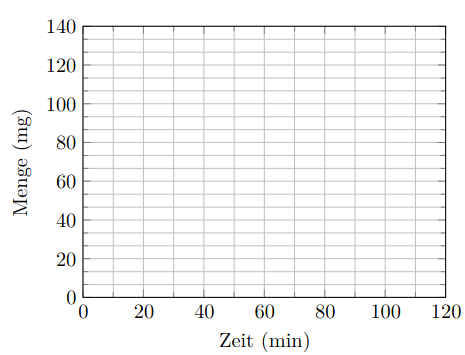
\includegraphics[width=150mm]{img/fct/Fct_ssA49.png}


c) Nach wie vielen Minuten ist die halbe Sättigungsmenge erreicht?}%% end deu

\eng{
  a) What is the value of $y$ for $x$ = 0 (initial value) and for $x\rightarrow \infty$ (saturation value)?

  b) Create a graph for $0 \le{} x \le{} 120$.
  
  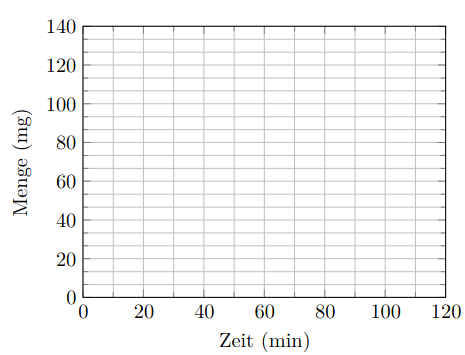
\includegraphics[width=150mm]{img/fct/Fct_ssA49.png}

c) In how many minutes is half of the saturation amount reached?
}%% end eng
\kVerweiseAltesKompendium{33}{50}
\kPlatzFuerBerechnungen{6}

}{%% Lösung

a) $f(0) = 0$ mg

   $\lim_{x\rightarrow\infty} (f(x)) = 125 $ mg  ($\lim$ = lat limes))

b) Grafik:

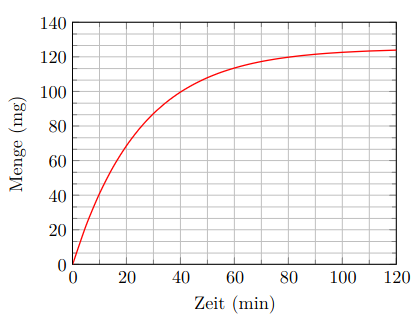
\includegraphics[width=150mm]{img/fct/Fct_ssL49.png}


c) \deu{Nach ca. 17.33 Minuten.}\eng{After about 17.33 minutes.}

}%% end Aufgabe


%% %%%%%%%%%%%%%%%%%%%%%%% Aufgabe %%%%%%%%%%%%%%%%%%%%%%%%%%%%%%%%%%%%%%%%%%%%%%%%


\kNiveauAufgabe{
\deu{Die Anzahl mg eines durch Infusion verabreichten Medikaments im Blut verläuft gemäss der
Funktion ($x$ = Anzahl Stunden ab Infusionsbeginn, $y$ = Anzahl mg
Medikament im Blut):}%% end deu
\eng{The number of milligrams of a medication administered through infusion in the blood follows the function ($x$ = number of hours since the start of the infusion, $y$ = number of milligrams of medication in the blood):}%% end eng


$$f : y = -250 \cdot{} e^{-0.2\cdot{}x} + 250$$


\deu{a) Stellen Sie die Funktion grafisch dar ($0 \le x \le 24$).

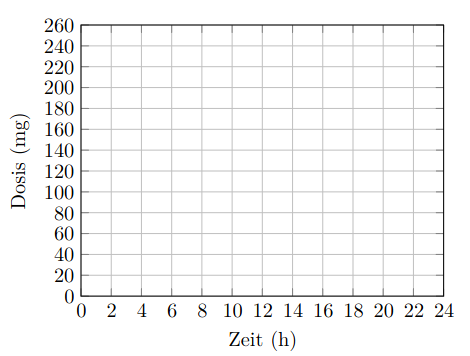
\includegraphics[width=150mm]{img/fct/Fct_ssA50.png}


b) Wie gross sind die $y$-Werte nach 3 und nach 4 Stunden ab
Infusionsbeginn?

c) Bei einer Dosis von 200 mg beginnt die Patientin plötzlich allergisch zu reagieren, worauf
die Infusion abgebrochen werden muss. Nach wie vielen Stunden ab Infusionsbeginn ist
dies der Fall?}%% end deu

\eng{a) Graphically represent the function ($0 \le x \le 24$).

  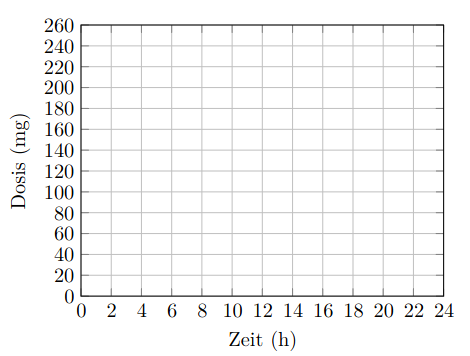
\includegraphics[width=150mm]{img/fct/Fct_ssA50.png}
  
b) What are the $y$ values after 3 and 4 hours from the start of the infusion?

c) With a dose of 200 mg, the patient suddenly starts to have an allergic reaction, leading to the termination of the infusion. After how many hours from the start of the infusion does this occur?}%% end eng

\kVerweiseAltesKompendium{34}{51}
\kPlatzFuerBerechnungen{6}


}{%% Lösungen

a)
\deu{Grafik:}\eng{Graphic:}

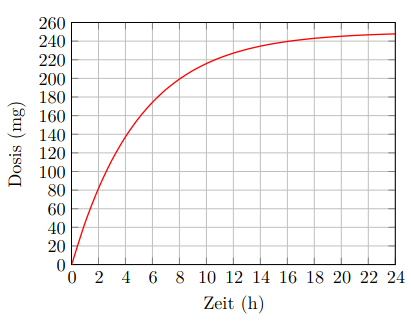
\includegraphics[width=150mm]{img/fct/Fct_ssL50.png}

b) $f(3)\approx 113$ mg \hspace{4cm}  $f(4) \approx{} 138$ mg

c) \deu{Nach 8.043 Stunden.}\eng{After 8.043 hours.}
 
}%% end Aufgabe

\newpage%% end chapter
